\chapter{Istniejące rozwiązania}

W niniejszym rozdziale przedstawione zostały wybrane z istniejących rozwiązań wspierających komunikację pomiędzy zawodnikami. Dla poszczególnych platform zostaną wyszczególnione ich główne założenia oraz sposób w jaki realizują cele podobne systemu będącego przedmiotem tej pracy.


\section{Facebook}

Facebook jest serwisem społecznościowym zrzeszającym prawie 2 miliardy osób z całego świata. Główną misją Facebooka jest zbliżanie do siebie ludzi poprzez umożliwianie budowy społeczności \cite{fb}.

Społeczność osób uprawiających sporty zespołowe nie stanowi tutaj wyjątku. Na Facebooku istnieje bardzo dużo grup tematycznych, których celem jest gromadzenie osób uprawiających pewną dyscyplinę sportu w określonym regionie. Osoby szukające osób do gry bardzo często tworzą posty podając takie informacje jak miejsce oraz termin spotkania, preferowany wiek oraz poziom umiejętności. Chętne osoby zgłaszają się pod postem lub poprzez wiadomość prywatną. Przykładowy post został przedstawiony na rysunku \ref{fig:ss-fb}.

Szukanie osób do gry poprzez portal Facebook jest bardzo często wybieranym rozwiązaniem głownie ze względu na dużą ilość użytkowników oraz szeroką dostępność serwisu. W tabeli \ref{tab:fbgrupy} przedstawiono zestawienie wybranych z publicznych grup w mieście Wrocław


\begin{table}[htb]
\centering\small
\caption{Przykładowe grupy dla zawodników na Facebook - stan z dnia 20.11.2018r}
\label{tab:fbgrupy}
\begin{tabularx}{\linewidth}{|p{.55\linewidth}|X|}\hline
Nazwa grupy & Liczba członków \\ \hline\hline
Piłka nożna Wrocław & 4689  \\ \hline
Siatkówka Wrocław & 4460  \\ \hline
Koszykówka Wrocław & 1686 \\ \hline
Piłka nożna Wrocław - dla PWR & 273  \\ \hline
\end{tabularx}
\end{table}


\begin{figure}[H]
\centering

\includegraphics[width=0.6\linewidth]{02-istniejace-rozwiazania/rys/ss-fb.PNG}
\caption{Przykładowy post użytkownika szukającego towarzyszy do gry na portalu Facebook}
\label{fig:ss-fb}
\end{figure}


\section{Playarena.pl}

Playarena.pl jest polskim portalem skierowanym do drużyn piłki nożnej 6 osobowej. Celem twórców jest zachęcanie ludzi do gry, dostarczanie możliwości rywalizacji, rozwoju oraz zabawy \cite{playarena}. Portal obecnie działa w wielu dużych miastach na terenie Polski, a użytkownicy mogą zgłosić propozycje nowych miast.

Po rejestracji w systemie użytkownicy mogą zakładać swoje drużyny lub dołączać do istniejących poprzez system aplikacji oraz zaproszeń. Skompletowane drużyny mogą uczestniczyć w rozgrywkach ligowych oraz w meczach towarzyskich. W przypadku drugiej kategorii kapitanowie drużyn mogą albo rzucić wyzwanie innej drużynie, albo zgłosić mecz do puli - inna drużyna może wtedy go podjąć. Użytkownicy mogą również dodawać oraz weryfikować obiekty sportowe.  


\section{SportsMatchMaker.com.au}

SportsMatchMaker jest Australijską siecią służącą do komunikacji pomiędzy sportowcami \cite{smmau}. Umożliwia nawiązywanie kontaktów w celu tworzenia drużyn oraz rywalizowania między sobą. Dodatkowo system posiada oraz rozwija bazę obiektów sportowych znajdujących się na terenie Australii. 

System umożliwia poszukiwanie osób uprawiających różne sporty, nie tylko zespołowe. Wyniki wyszukiwania można zawężać do wybranej lokalizacji w określonym zasięgu. Dodatkowo użytkownicy definiują swój poziom zaawansowania w danej dziedzinie. Komunikacja pomiędzy zawodnikami odbywa się za pomocą wiadomości prywatnych.


\begin{figure}[H]
\centering
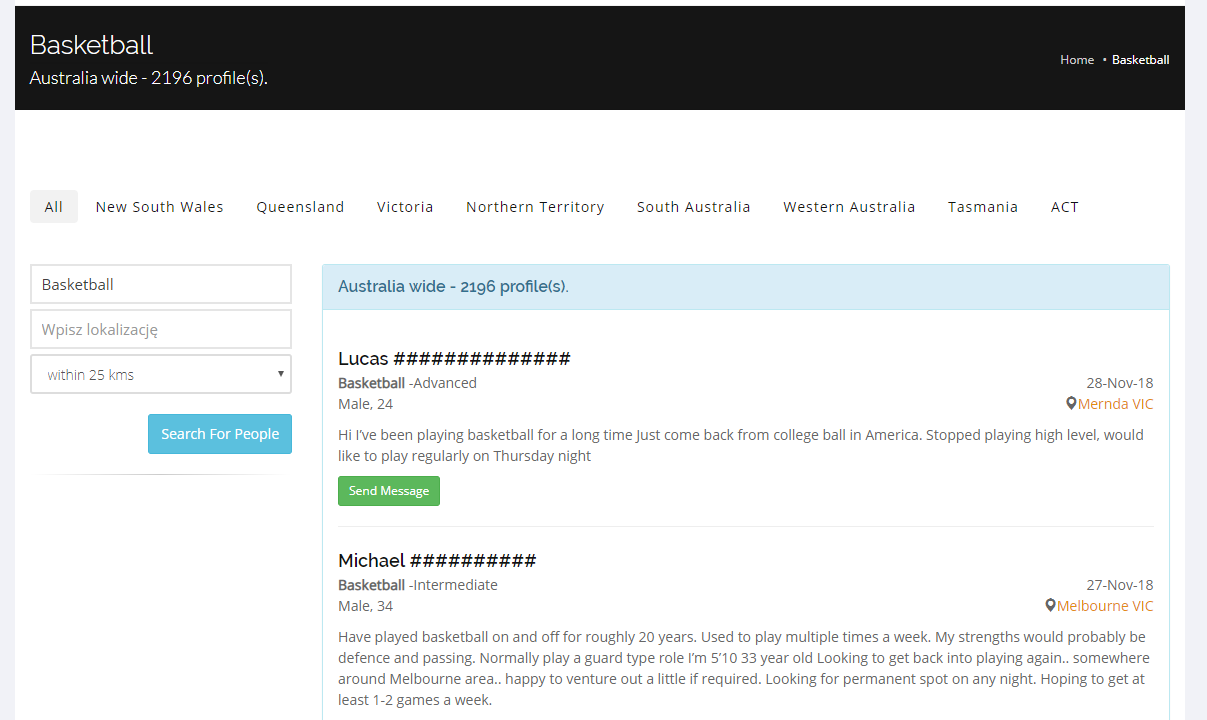
\includegraphics[width=\linewidth]{02-istniejace-rozwiazania/rys/ss-austr.PNG}
\caption{Przykładowe wyniki wyszukiwania osób grających w koszykówkę}
\label{fig:ss-austr}
\end{figure}